\chapter{Implementacja wielop�tlowego regulatora PID}

\section{Dobieranie nastaw PID}

\begin{figure}[h!b]
	\centering
	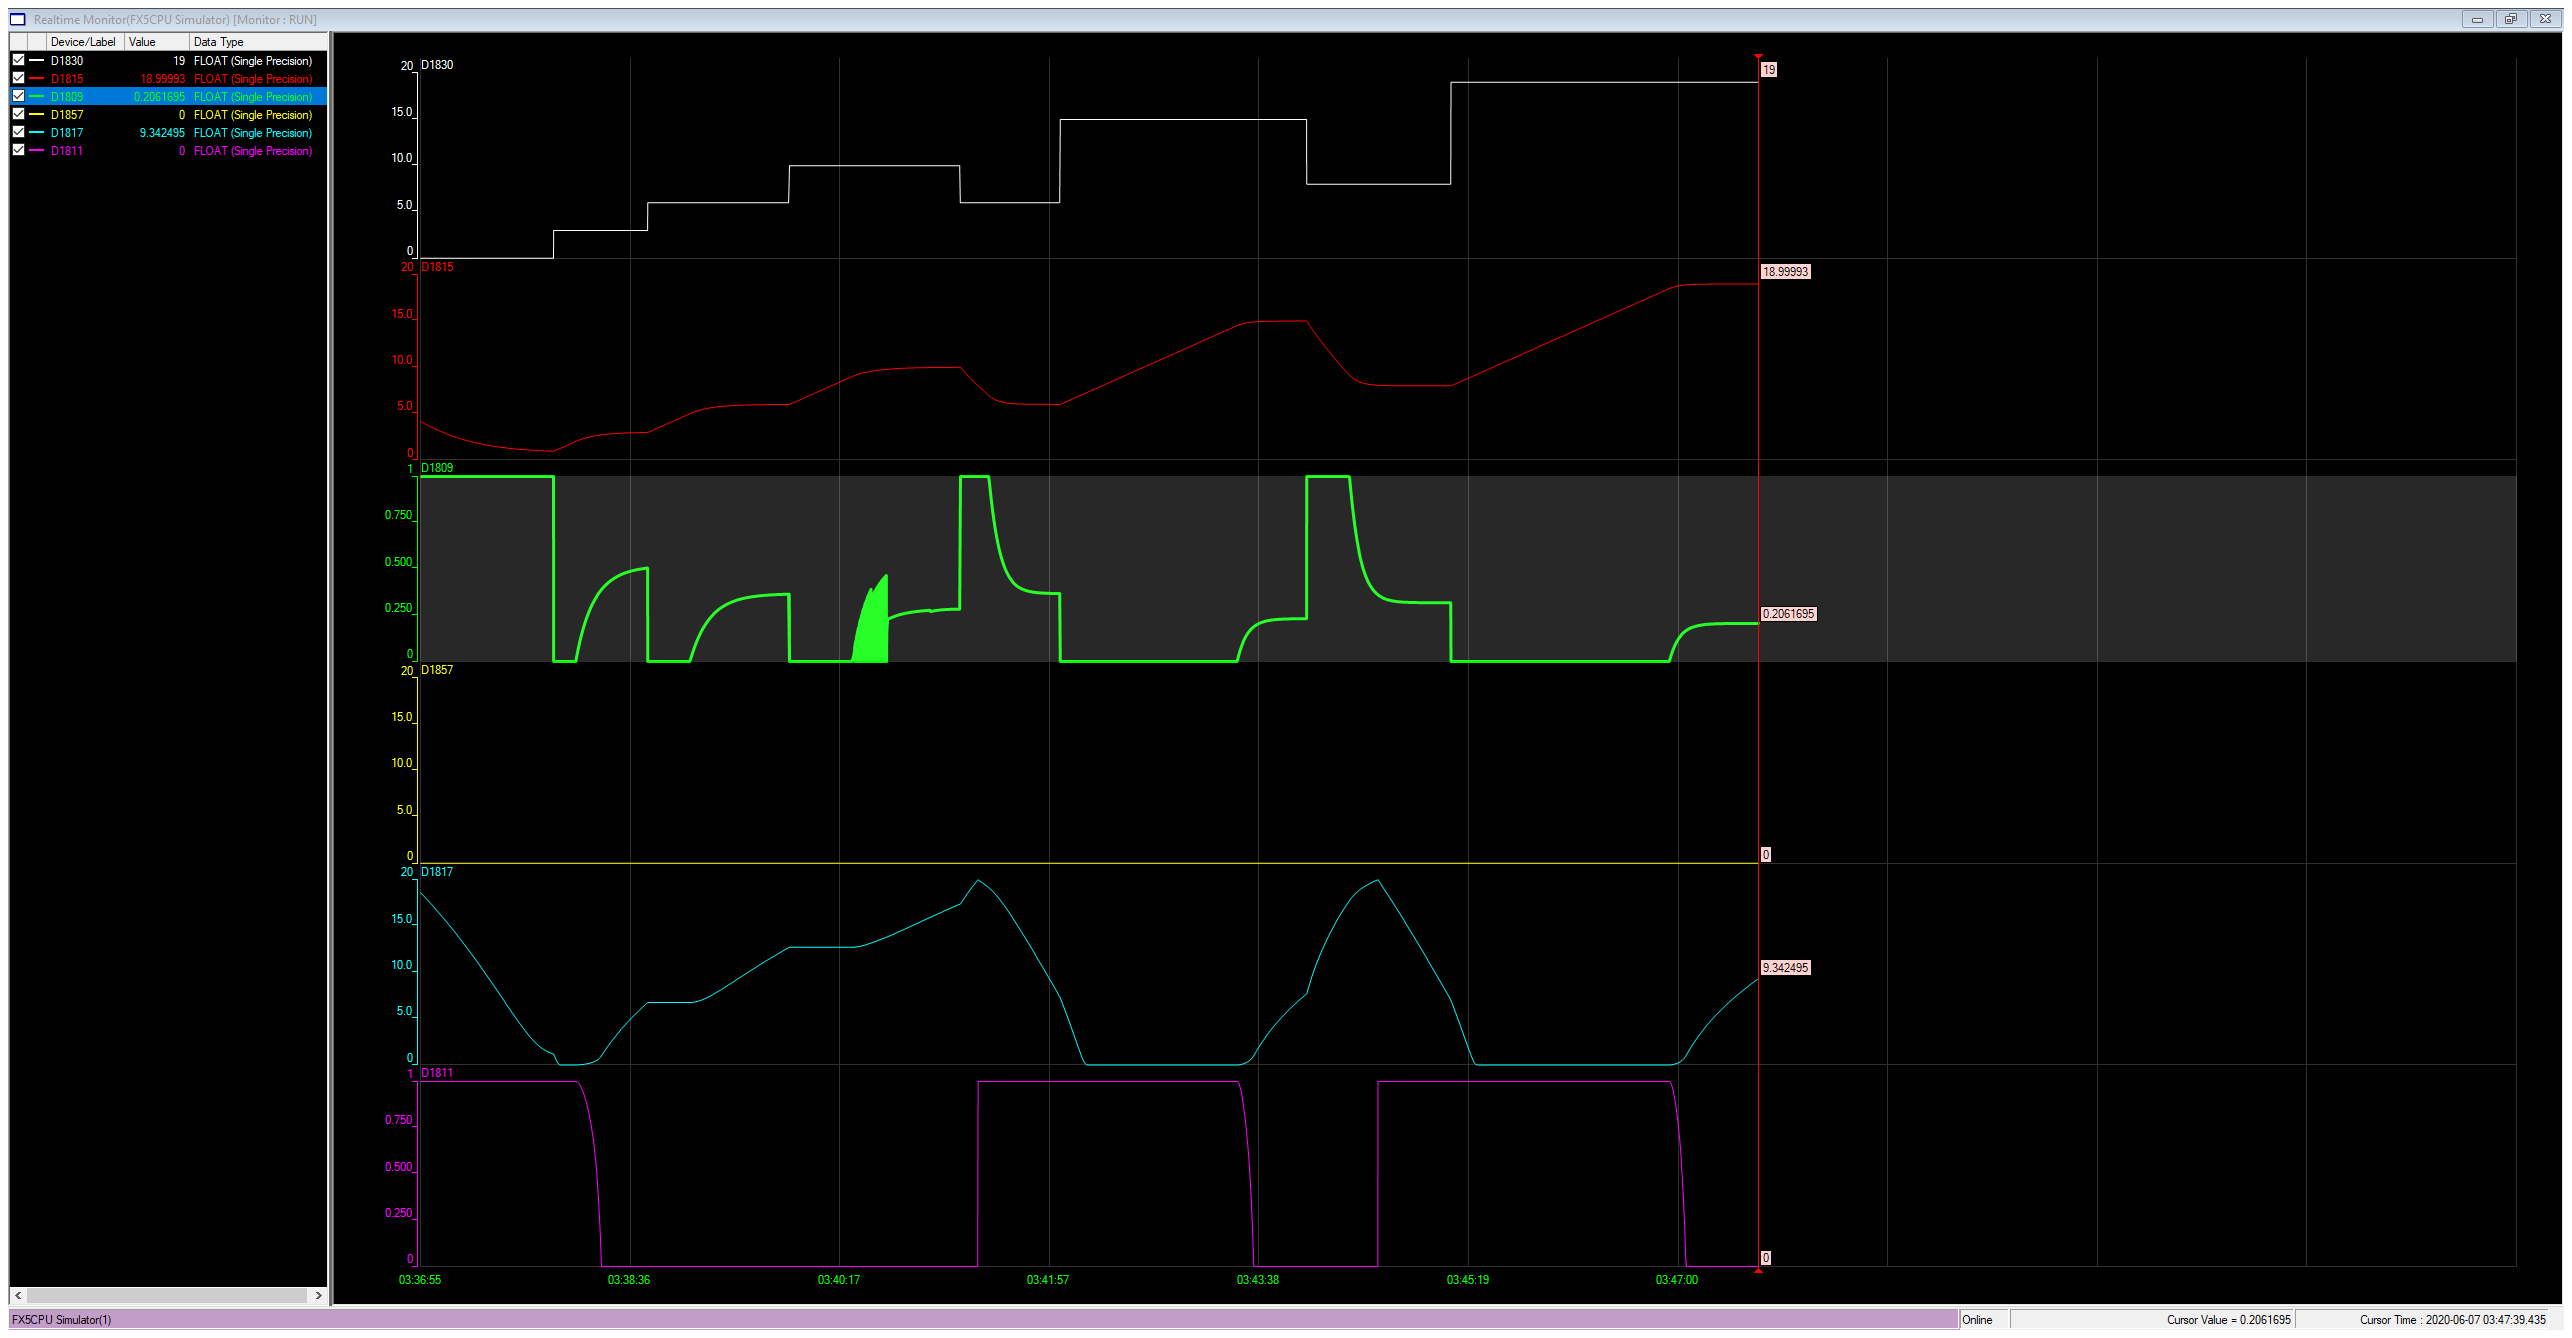
\includegraphics[clip, trim = 0 0 550 0, width=\textwidth, center]{rysunki/STROJENIE_PID_1.png}
	\caption{Wykres prezentuj�cy przebieg podczas strojenia}
	\label{strojenie_pid_1}
\end{figure}

ok k1 = -80, ti1 = 50

\begin{figure}[h!b]
	\centering
	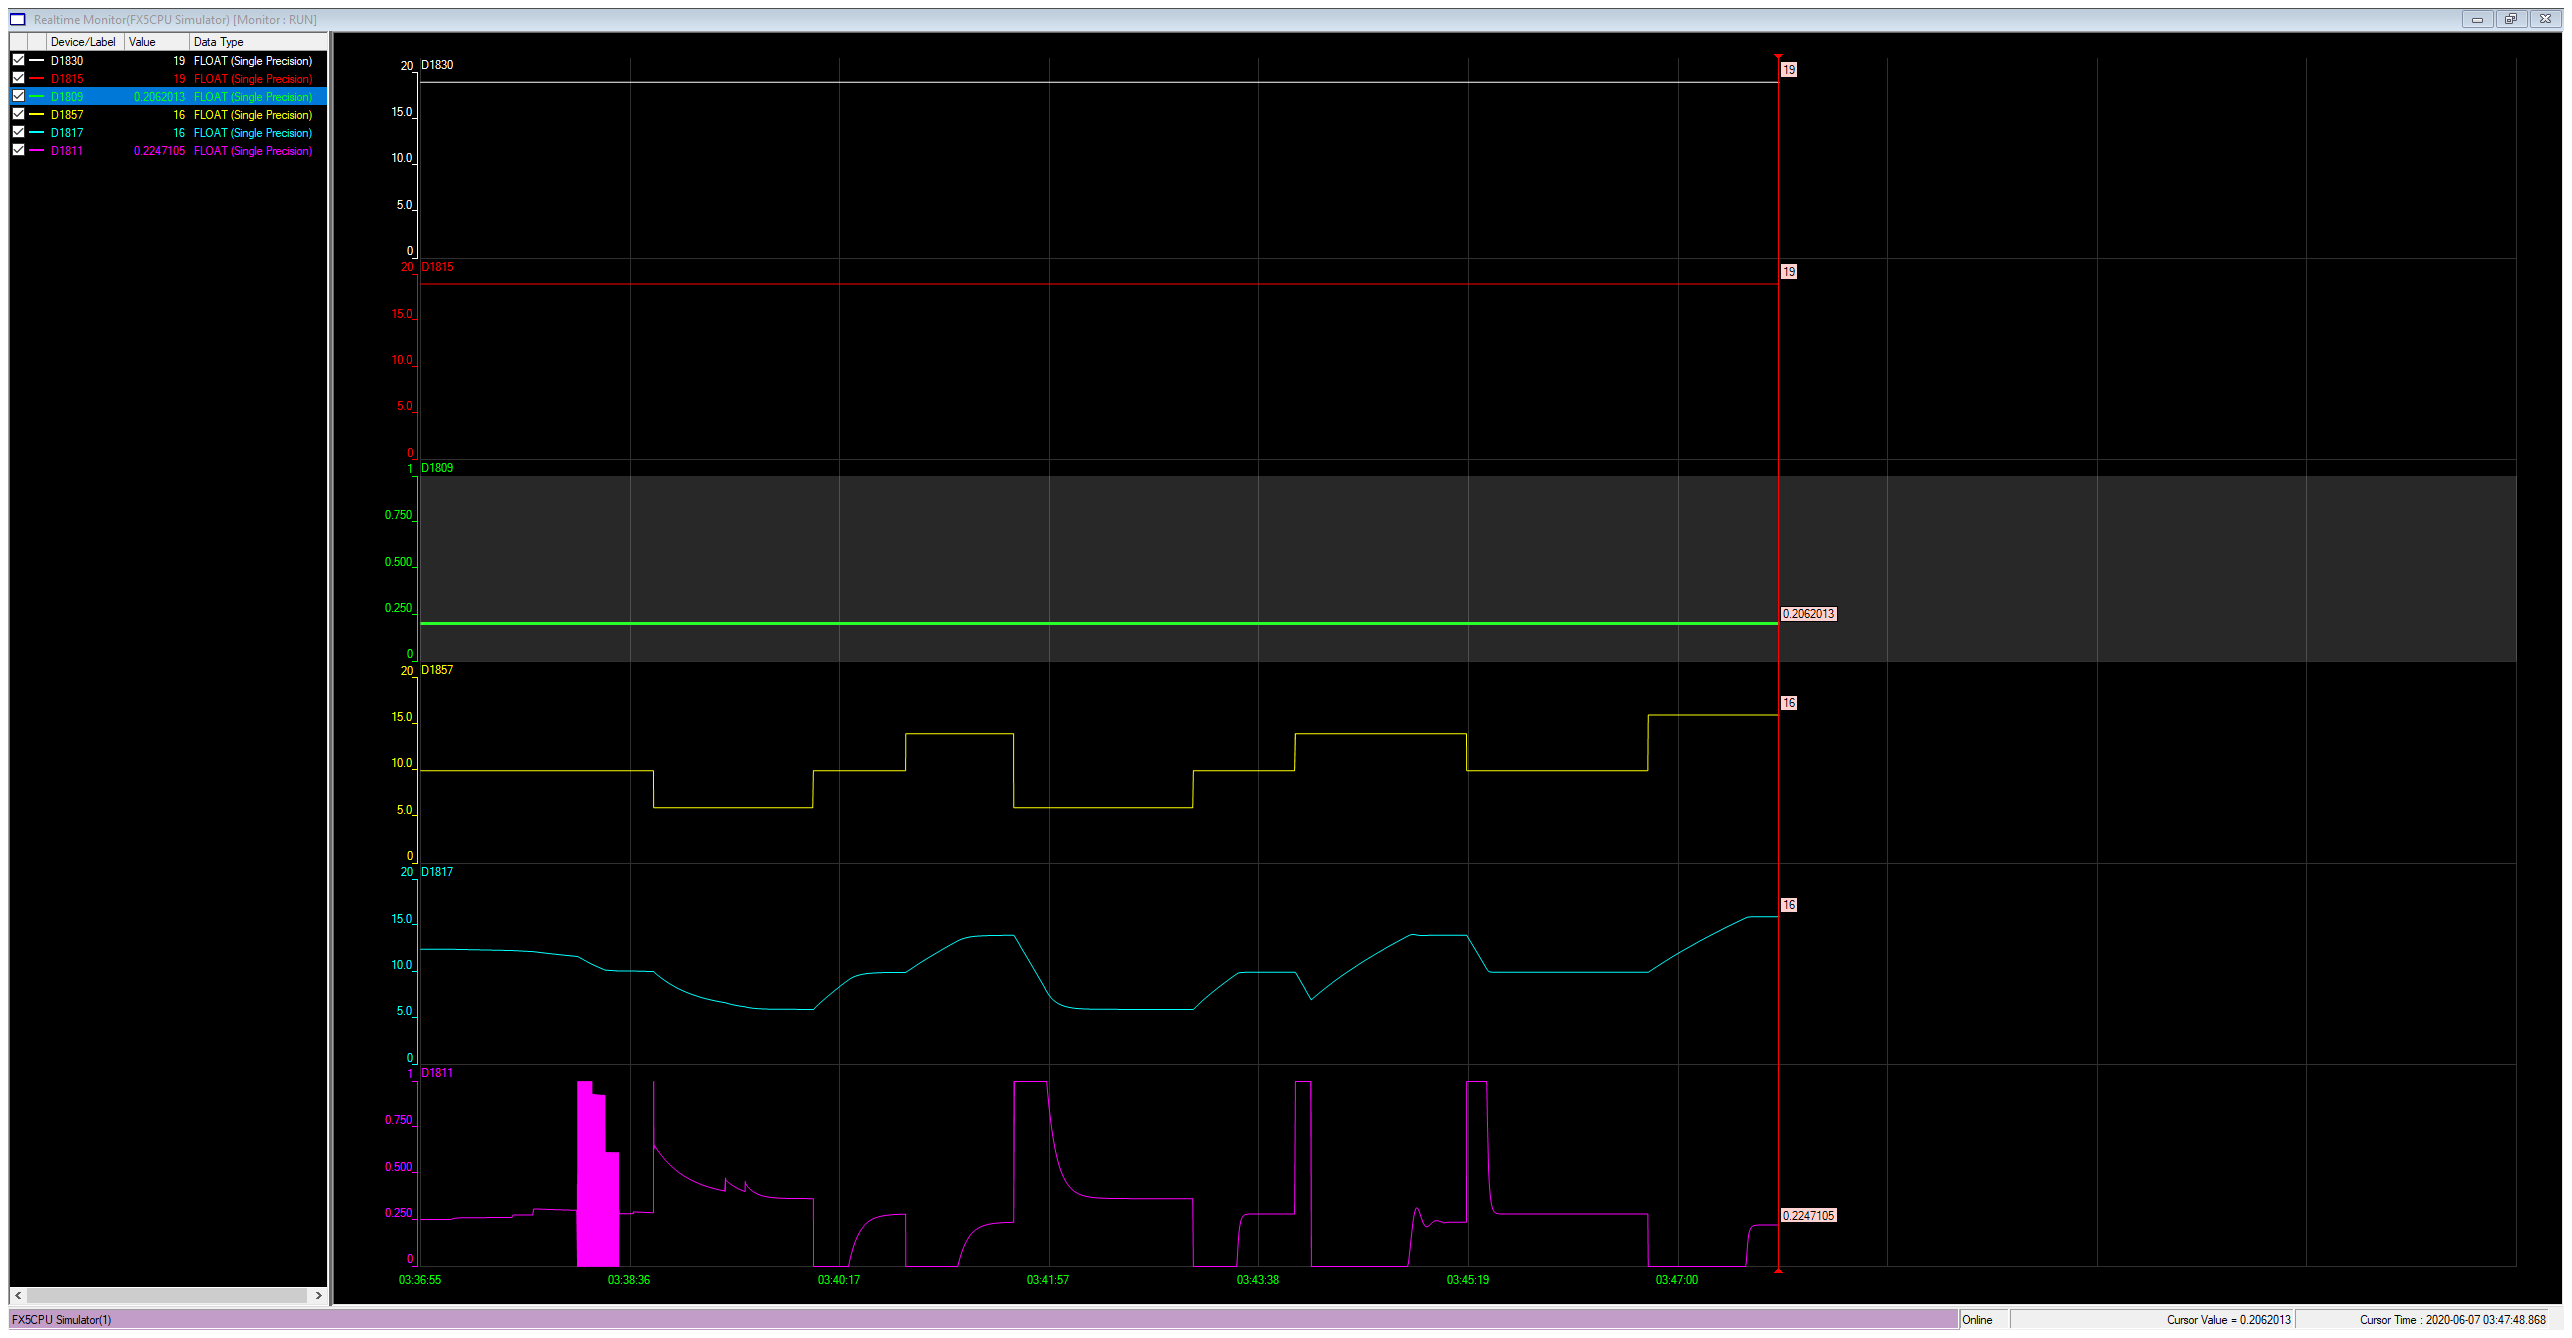
\includegraphics[clip, trim = 0 0 540 0, width=\textwidth, center]{rysunki/STROJENIE_PID_2.png}
	\caption{Wykres prezentuj�cy przebieg podczas strojenia}
	\label{strojenie_pid_2}
\end{figure}

ok k1 = -20, ti1 = 5 -> 1

\begin{figure}[h!b]
	\centering
	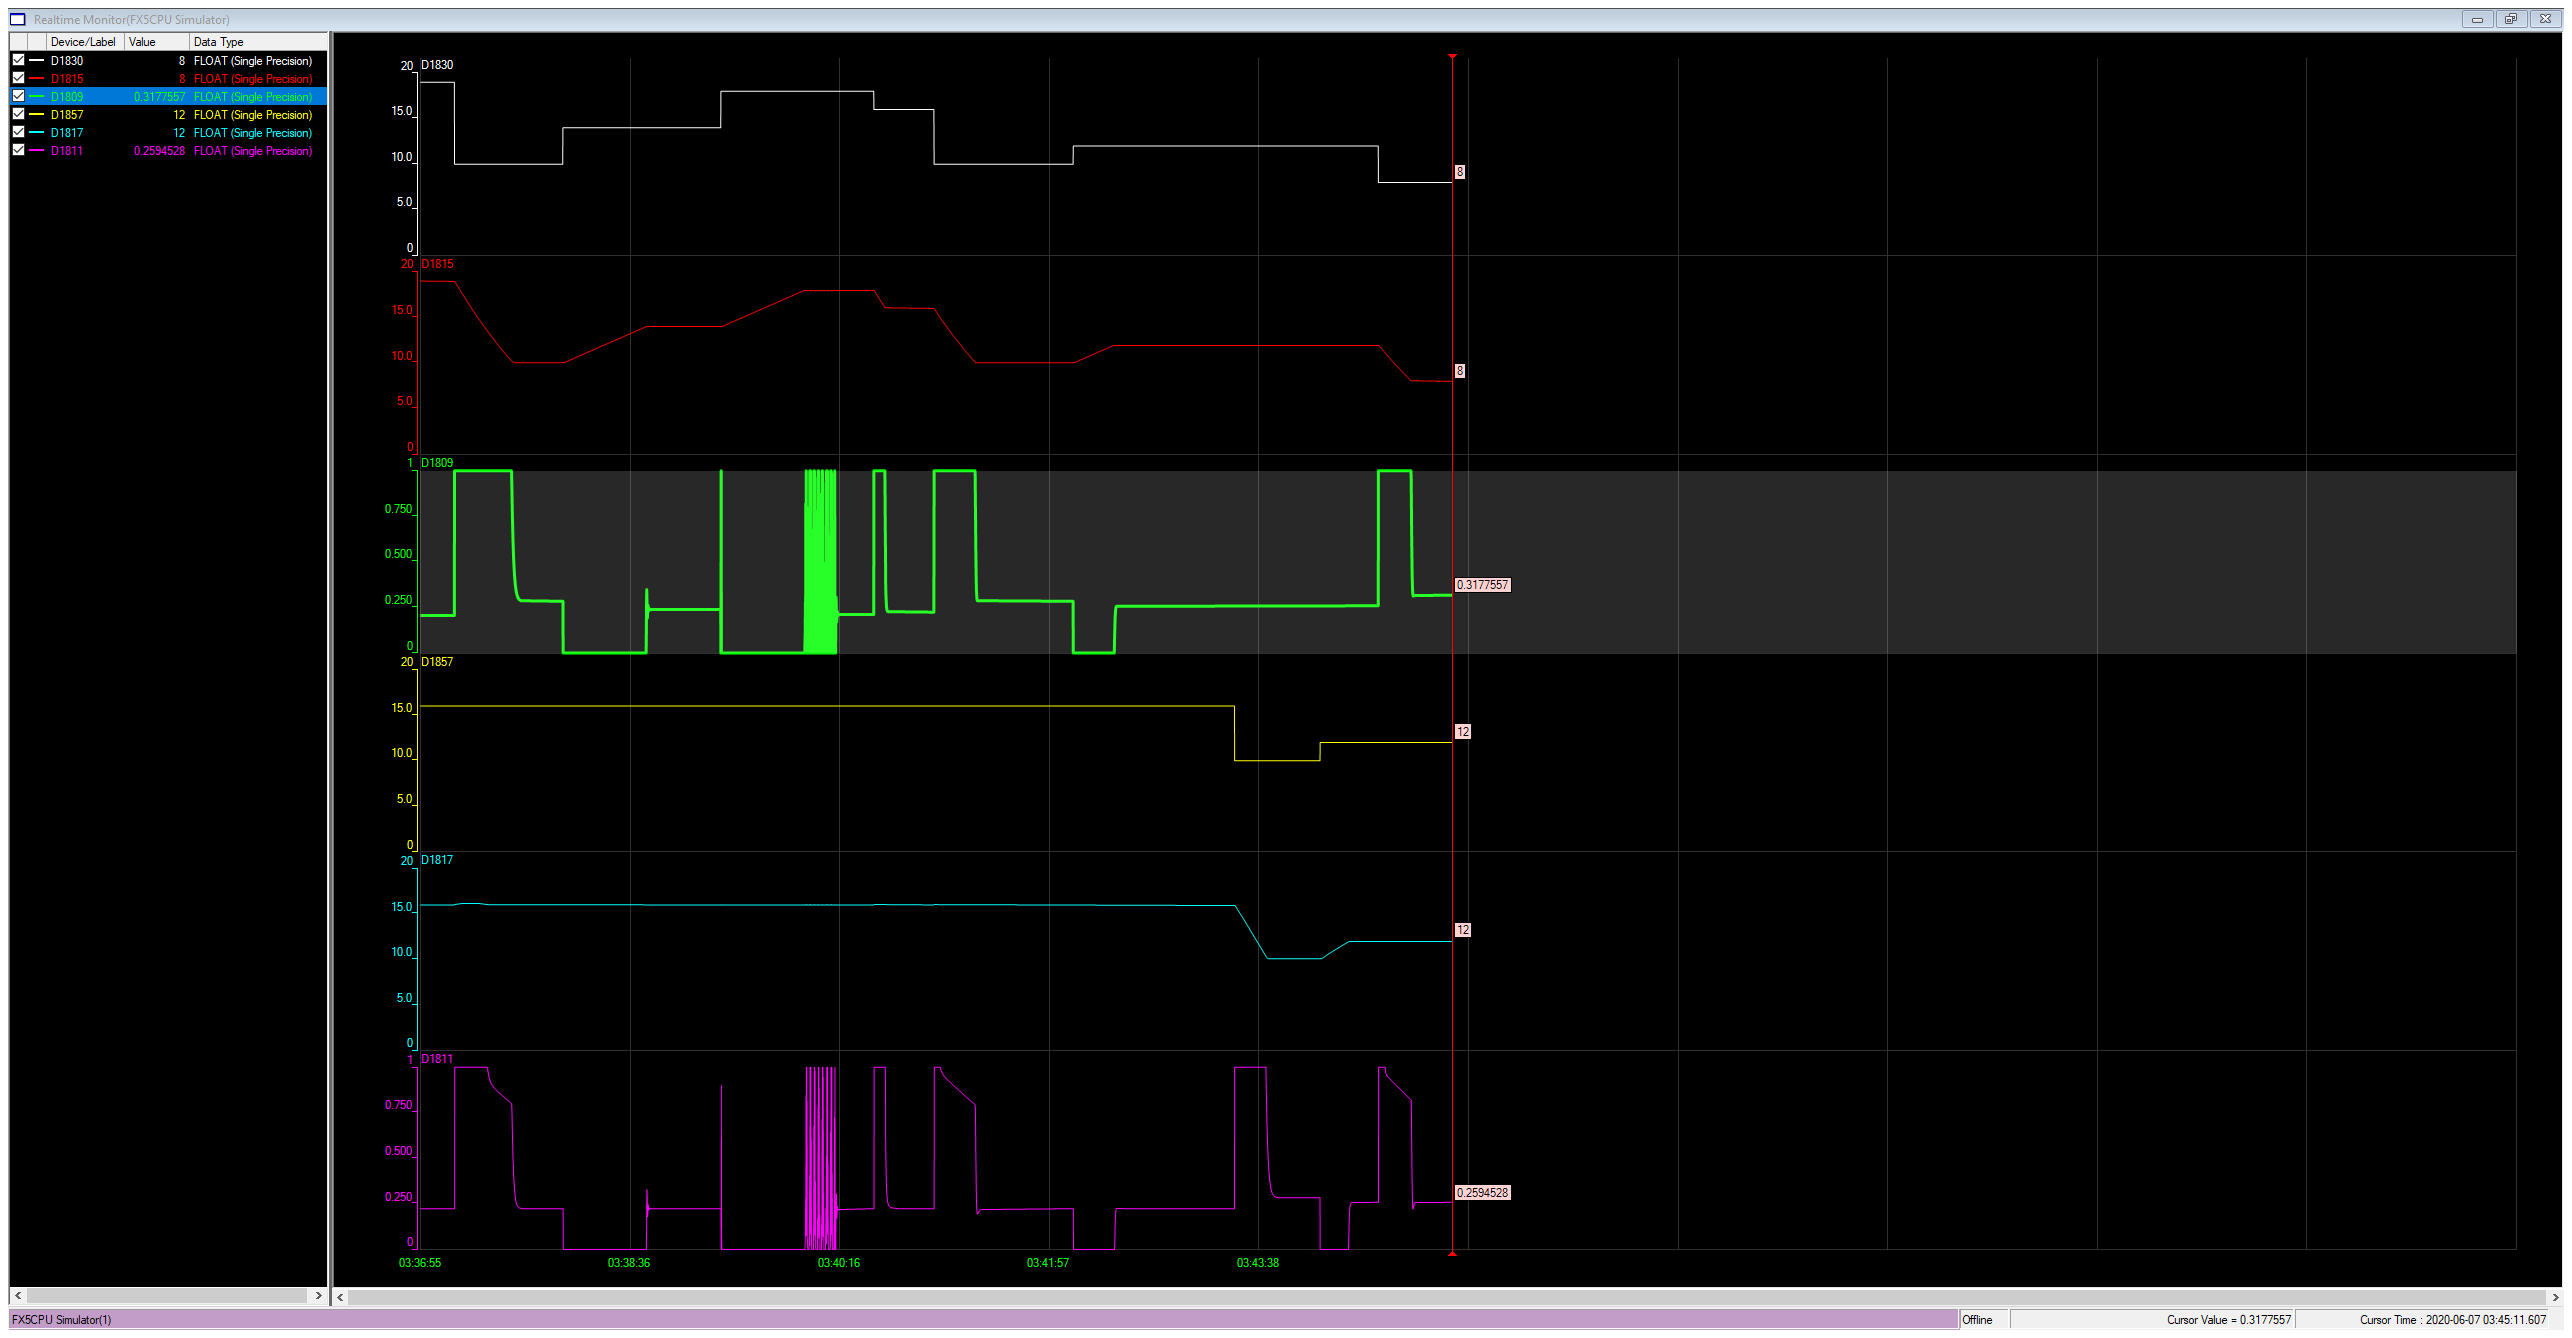
\includegraphics[clip, trim = 0 0 780 0, width=\textwidth, center]{rysunki/STROJENIE_PID_3.png}
	\caption{Wykres prezentuj�cy przebieg podczas strojenia}
	\label{strojenie_pid_3}
\end{figure}

k1 = -20 ti1 = 0.4